\begin{comment}
2.3 Teil II: SW-Projektdokumentation
Hier folgen die Dokumente gemäss Software-Engineering-Vorgehen.
2.3.1 Überblick
Zweck und Inhalt dieses Kapitels
2.3.2 Vision
Verweis auf Teil I.
2.3.3 Anforderungsspezifikation
Enthält folgende mögliche Unterkapitel:
 Rahmenbedingungen (wenn nicht schon oben abgehandelt)
 Anwendungsfalldiagramm
 Hauptanwendungsfall
 Funktionale Anforderungen
 Nicht-Funktionale Anforderungen
 Weitere: Aktivitätsdiagramme, Fallbeispiele, Szenarien, Prototypen...
2.3.4 Analyse
Klassen-, bzw. Domainmodell.
2.3.5 Design (Entwurf)
Die Architektur soll eine objektorientierte Problemdomain umfassen. Eine allfällig eingesetzte Datenbank darf diese Problemdomain permanent speichern, nicht aber ersetzen.
Enthält folgende mögliche Unterkapitel:
 Klassenverantwortlichkeiten (Klassenname, Verantwortlichkeit, Wissen, Tun, Abhängigkeiten); CRC- Diagramme?
 Sequenzdiagramm / Kollaborationsdiagramm
2.3.6 Implementation (Entwicklung)
Objektkatalog: könnte mit einem Thesaurus verwaltet werden! Rest individuell.
2.3.7 Test
Enthält folgende mögliche Unterkapitel:
 Testverfahren automatisch (mit JUnit) und manuell (dokumentiert; z.B. GUI); durchnummeriert.
 Iterationen 1 ... X
2.3.8 Resultate
Resultate und Ergebnisse der Arbeit. Dieser Abschnitt richtet sich an den speziell für das entsprechende Fachgebiet interessierten Ingenieur. Er soll es ihm ermöglichen, die für die Problemlösung gemachten Überlegungen zu verstehen und nachzuvollziehen.
2.3.9 Weiterentwicklung
Möglichkeiten der Weiterentwicklung: Funktionen und mögliches weiteres Vorgehen. Weiterentwicklung scheint allgemein ein heikler Punkt zu sein in allen Projekten, besonders auch in SA/DA-Projekten:
In realen Projekten, im RUP-Prozess wird er kaum betont und auch für Sie und für die Auftraggeber scheint es ein Problem zu sein. Warum?
 Wenn man dort zuviel aufschreibt, dann könnte das als Manko aufgefasst werden; und Aufschreiben nimmt erst noch Zeit weg...
 Zudem ist aus Sicht Auftraggeber (ohne "Gegensteuer") eine zusätzliche Funktion besser bewertbar als der "Wert" eines robusten, sauberen Designs oder eines Refactorings (z.B. der Separierung der Objekt/Klassen-Zuständigkeiten).
Ein Test, wie "sauber" - namentlich: wie änderungsfreundlich - ein Design ist, zeigt sich beispielsweise in der Antwort auf folgende Frage: "Welche Interfaces muss man implementieren und/oder welche Komponenten/Klassen muss man erweitern (schlimmstenfalls anpassen), um eine weitere Funktionalität einzubauen? Z.B. ein weiterer Exportfilter?".
Daher gelten folgende Regelungen zur Weiterentwicklung (gilt auch für andere Projektarten):
 Weiterentwicklung ist obligatorisch und erscheint in zwei separaten Kapitel (ggf. Dokument): Im Technischen Bericht, Unterkapitel Resultate/Ausblick, und in der SW-Projektdokumentation.
 Weiterentwicklung im Technischen Bericht ist allgemein gehalten und daher weniger heikel. Wichtig ist die Aufzählung der hauptsächlichen weiteren möglichen funktionalen oder nicht-funktionalen Anforderungen.
 Weiterentwicklung in der SW-Projektdokumentation ist an Architekten / SW-Entwickler gerichtet wie jedes andere SW-Dokument.
 Gewichtung: Es wird separat bewertet und zusätzlich erst spät (SA/DA bei der Präsentation) vollständig abgegeben wird. Spät heisst bei DAs auf der Dokumentation der Präsentation (inkl. CD). Sein ungewichtetes Gewicht gegenüber der Gesamtdokumentation ist umfangmässig ca. 1/15. Zur Erinnerung siehe Unterkapitel Lieferdokumente mit ca. 15 Hauptkapitel-/-Dokumenten.
2.3.10 Benutzerdokumentation
Installationsanleitung(en), Bedienungsanleitung(en) und Tutorien (evtl. in den Anhang)! Vergessen Sie a) nicht den CD-Inhalt zu notieren und auch in die Doku. zu nehmen.
Testen sie die Installation mit realistischen Vorgaben!!
2.4.1 Allgemeines
 Normen
 Konfigurationsmanagement (Entwicklungs-Werkzeuge, Eingesetzte Software)
2.4.2 Projektmanagement
Enthält folgende mögliche Unterkapitel:
 Vorgehen
 Zeitplanung
 (Erreichen der Ziele siehe sep. Kapitel "Bewertung und Ausblick").
Zeitplanung: Die Zeitplanung orientiert sich an den Meilensteinen und ist nach folgender Idee strukturiert:
     Inception => Elaboration => Construction 1 => Construction 2 => ... => Transition
Das ergibt folgendes Zeitdiagramm:
2.4.3
                          Dokumente
Dokumente Teil I:             |
+ Einführung                  |
+ Vision                      |
+ "Stand der Technik"         |
+ Umsetzungskonzept           |
+ Resultate                   |
Dokumente Teil II:            |
+ Anforderungsspezifikation   |
+ Analyse                     |
+ Design                      |
+ Implementation              |
+ Projektmgmt.&-Monitoring    |
+ Test                        |
+ Resultate und Weiterentw.   |
+ Benutzerdokumentation       |
+ Glossar und Abkürzungsverz. |
+ Literatur- und Quellenverz. |
                              +----+------+---------+---------+------> Tage
               Zeitabschnitte: Inc.  Elab.  Constr.1  Constr.2  Trans.
Projektmonitoring
Code-Analyse (Metriken).
\end{comment}

\part{Projektdokumentation}

\chapter{Vision}

\chapter{Anforderungen}
\section{User Stories}
\subimport{}{userstories.tex}

\section{Nicht-funktionale Anforderungen}


\chapter{Analyse}
\section{Plugins}
\subsection{jsLint}

\chapter{Design und Implementation}


\section{Architektur}

Daten-Lieferanten liefern ihre Daten per Web-Interface oder REST-Api. Diese Daten werden in der Datenbank gespeichert und im Web-Interface angezeigt. Daten-Nutzer rufen diese Daten wieder über das Web-Interface oder per REST-Api ab. 

Dritt-Entwickler können eigene Komponenten entwickeln und beisteuern, wie in \cref{fig:arch-overview} zu sehen ist:
\begin{description}
\item[Parser] nehmen Daten entgegen und bereiten sie zur Weiterverarbeitung auf
\item[Formatter] formattieren Daten in das vom Benutzer gewünschte Format
\end{description}

\begin{figure}[H]
    \centering
    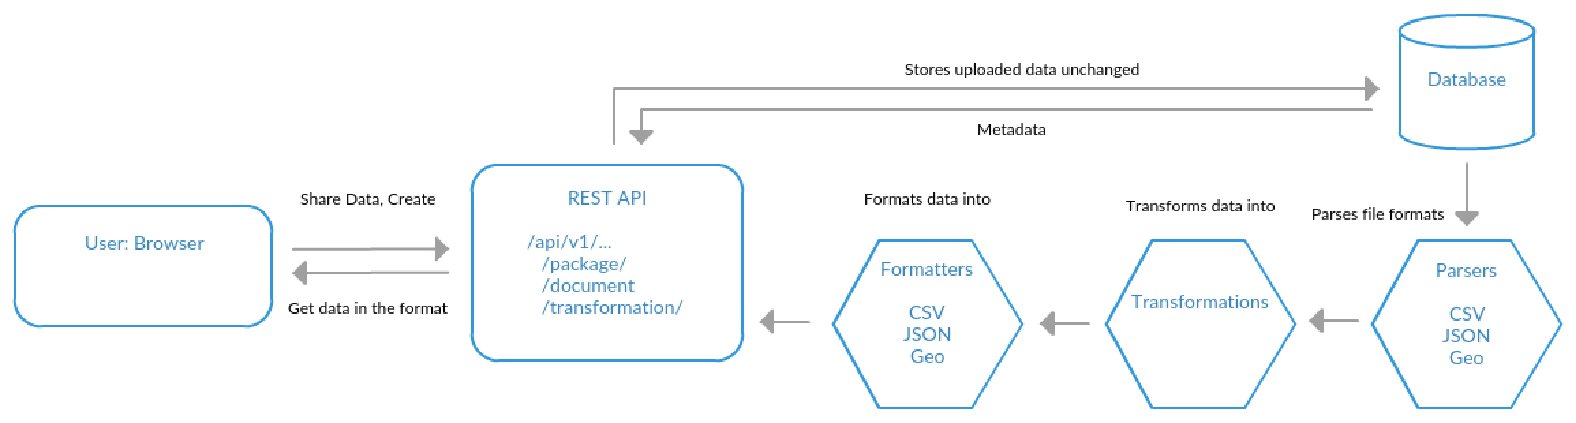
\includegraphics[width=\linewidth]{fig/ODH-Architecture-Overview}
    \caption{Grobe Architektur-Übersicht}
    \label{fig:arch-overview}
\end{figure}

\subsection{Datenspeicherung}
Ein Ziel dieser Arbeit ist die Erstellung eines Daten-Hubs, welcher es Anbietern ermöglicht, ihre Daten anderen zur Verfügung zu stellen. Zur Speicherung der Daten stehen folgende Varianten zur Auswahl.

\subsubsection{File-basiert}
Die Daten werden direkt im Datei-System gespeichert. Um Konflikte zwischen Datei-Namen zu vermeiden muss ein Hashing-Schema definiert und verwendet werden. Metadaten zu den Dokumenten werden in einer Datenbank hinterlegt.

Die Daten werden in ihrem Ursprungsformat belassen, bis ein Nutzer eine Transformation auswählt und anwendet. Die Resultate einer solchen Transformation können direkt wieder im Datei-System gecached werden um weiter Abfragen nach der selben Transformation zu beschleunigen.

Die Tatsache, dass die Daten im Datei-System liegen vereinfacht die Einbindung von Software von Drittanbietern.

Ein Nachteil dieser Variante ist, dass Cloud-Anbieter wie Heroku keine schreibbaren bzw. keine beständigen Dateisysteme anbieten, sondern auf die Verwendung von Amazon S3 oder ähnlich verweisen.\footnote{siehe \url{https://devcenter.heroku.com/articles/read-only-filesystem} bzw. \url{https://devcenter.heroku.com/articles/dynos\#ephemeral-filesystem}}

Metadaten sollten weiterhin in einer Datenbank gehalten werden.

\subsubsection{Datenbank-basiert, einzelne Records}
Die Daten werden in einzelne Records zerlegt und zusammen mit den Metadaten in einer Datenbank gespeichert. Dies erfordert, dass bereits der Daten-Anbieter eine Transformation in das Record-Format auswählen muss. Falls sich herausstellt, dass dies zu langsam ist um es direkt im HTTP-Request des Anbieters durchzuführen, müssen die Daten vor der Transformation zwischengespeichert werden.

Falls die Transformations-Resultate auf der Nutzer-Seite gecached werden sollen ist eine weitere Datenablage für die Transformationsresultate notwendig.

Die Einbindung von Drittanbieter-Software erfordert mehr Aufwand, falls diese nur auf Dokumenten- oder gar Datei-Ebene arbeiten.

Laut \prof wird diese Version bereits von diversen Schema Mapping-Tools verwendet (\gls{kettle}, \gls{fme}).

\subsubsection{Datenbank-basiert, Dokument als Blob}
Die Daten werden ohne Transformation zusammen mit den Metadaten in einer Datenbank abgelegt. Diese Variante hat praktisch alle Vorteile der File-basierten Version.

Falls Dritt-Anbieter-Software nur auf Datei-basis arbeitet kann ein temporäres oder flüchtiges Datei-System verwendet werden.

Für diese Variante existieren folgende Möglichkeiten:
\begin{description}
\item[Daten und Metadaten in der selben Tabelle] Daten und Metadaten werden in der selben Tabelle gespeichert. Dies bietet ein einfacheres Schema, erlaubt jedoch nur ein Daten-Objekt pro Dokument, was ungeeignet ist für Dokument-Typen wie ESRI Shapefile, welche aus mehr als einer Datei bestehen.
\item[Daten und Metadaten in separaten Tabellen] Daten und Metadaten werden in unterschiedlichen Tabellen gespeichert. Dies erlaubt die Speicherung von Dokumenten bestehen aus mehreren Dateien, oder transformierten Daten als zusätzlichen Daten-Eintrag zu einem Metadaten-Record. Dies erlaubt es auch, Django-Models zu erstellen welche nicht jedes mal die Daten abfragen, obwohl nur Metadaten benötigt werden.
\end{description}

\subsubsection{Fazit}
Die Speicherung von Daten auf Record-Basis weist unserer Meinung nach diverse Nachteile auf: 
\begin{itemize}
\item Es setzt eine Transformation voraus, welche die Daten ``flachklopft''. Dies kann verlustbehaftet sein.
\item Die Transformation muss bereits beim Hochladen der Daten zur Verfügung stehen.
\end{itemize}

\xxx[document decision to support cloud service providers/heroku]
Wir entschieden uns bereits zu einem früheren Zeitpunkt, zu Cloud-Anbietern, insbesondere Heroku, kompatibel sein zu wollen. Da bei der File-basierten Version ausserdem neben dem File-Backend trotzdem noch eine Datenbank verwendet wird, entschieden wir uns für einen Datenbank-basierten Ansatz.

Um Dokument-Typen wie ESRI Shapefile einfacher unterstützen zu können kommt die Version mit separaten Tabellen für Daten und Metadaten zum Einsatz.

\subsection{Komponenten}


\subsection{Klassen}


\subsection{Sequenzdiagramm}



\section{User Interface}
\subsection{Authentifizierung}
Zur Authentifizierung der Benutzer wird der oAuth 2 Standard verwendet. Dieser erlaubt ein Login mit einem GitHub, FaceBook oder anderem Konto. Implementiert wurde dieser Standart auf der REST Seite mit hilfe von verschiedenen Django Plugins. 
Beispielsweise wurde python-social-auth verwendet um den Benutzer gegenüber diesen Diensten zu authentisieren. Die REST Schnittstelle wird dann über einen Token gesichtert.


\section{Testing}


\chapter{Resultate und Ausblick}

\section{Resultate}


\section{Weiterentwicklung}


